\documentclass[twoside]{article}
\usepackage[utf8]{inputenc}
%\usepackage[uebung, answers]{tumbgdm}
\usepackage[uebung]{tumbgdm}
\usepackage{lecturesetup}
\nummerUebungsblatt{1}
\nummerErsteFrage{1}

\LearningOutcome{
You learn how to use MATLAB, you learn to know basic loops and how to write functions with and without arguments. You accomodate yourself with variables, global variables, and state updates through the turtle graphics mechanism.
}

\begin{document}
\maketitle


\begin{task}{Basics in MATLAB}{}{}
In this task, we want to practice  certain elements of the MATLAB language which you will find helpful when trying to write your first programs. This includes

- Types and variables
- Casting
- Matrices

Recall all numeric data types of the MATLAB language as can be found in the official MATLAB manual (\url{https://de.mathworks.com/help/matlab/numeric-types.html}). Then try to answer the following questions and complete the following program snippets.

\begin{enumerate}

\item{\textbf{Some Casting:} Look up casting here \url{https://www.mathworks.com/help/matlab/ref/cast.html}. Then cast the number given by $\pi$ multiplied with 100 to int32, int8 and uint8. What is happening when you cast to int8 and uint8?
}

\item{\textbf{Some Rounding:} Implement a small script in which one variable is set to 2.4 and another variable is set to 42. Compute the sum of both and round it up and down to the nearest integer. Store the result in variables called \code{sum\_rounded\_up} and \code{sum\_rounded\_down}. For that, you can either use typecasting between floating point and integer numbers which typically truncates numbers or you can have a look at dedicated functions such as \code{ceil}, \code{floor}, \code{round}. See as well \url{https://de.mathworks.com/help/matlab/ref/round.html}.}


\item{\textbf{Identity Matrix:} Create the following matrix. Do this by hand or using the the eye function (https://de.mathworks.com/help/matlab/ref/eye.html).
  \[
  I= \begin{pmatrix}
    1 & 0 & 0\\
    0 & 1 & 0\\
    0 & 0 & 1\\
\end{pmatrix}
  \] \emph{Optional: When you come back to this task after learning loops, try to write a custom eye function yourself.}
  }

\item{\textbf{Some Slicing:} Given the matrix M with 8 columns and 6 rows, extract each evenly numbered row and compute the sum.
  \[
  M= \begin{pmatrix}
1 & 2 & 3 & 4 & 5 & 6 & 7 & 8\\
11 & 12 & 13 & 14 & 15 & 16 & 17 & 18\\
21 & 22 & 23 & 24 & 25 & 26 & 27 & 28\\
31 & 32 & 33 & 34 & 35 & 36 & 37 & 38\\
41 & 42 & 43 & 44 & 45 & 46 & 47 & 48\\
51 & 52 & 53 & 54 & 55 & 56 & 57 & 58\\
\end{pmatrix}
 \]
}

\item{\textbf{Matrix Multiplication:}
Find out how to multiply two matrices and compute the multiplication of the following matrices $A$ and $B$.
\[
  A= \begin{pmatrix}
1 & 2 & 3\\
3 & 2 & 1\\
\end{pmatrix}
B= \begin{pmatrix}
1 & 2 \\
3 & 3 \\
2 & 1
\end{pmatrix}
\]
}
\item{\textbf{Matrix Inversion:} Look up the documentation for matrix inversion (\url{https://www.mathworks.com/help/matlab/ref/inv.html}) and invert the matrices above (when possible).}

\item{\textbf{Linear System Solving:} In order to solve the following system of linear equations given as an $n \times n$ square matrix $A$ an (row-)vector of $n$ unknown numbers, and a (row-)vector of $n$ known numbers (e.g., measurements) $b$

\[
Ax =b
\]
MATLAB provides a very nice syntactic feature in which you can write the inversion of the system as a "right-division". Find out, how to do this and compute the solution of the system using MATLAB.

\[
A =\begin{pmatrix}
1 & 2 \\
3 & 4
\end{pmatrix}
b=\begin{pmatrix}
1 \\
1
\end{pmatrix}
\]
The advantage of this notation over an approach in which one computes an inverse matrix $A^-1$ such that $A\cdot A^{-1} = A^{-1}\cdot A = I$ with $I$ being the identity matrix and computing
\[
  Ax = b \Leftrightarrow x = A^{-1}b
  \]
  is that MATLAB can choose the best algorithm based on the properties of $A$. Inverting the matrix can be numerically unstable, such that an algorithm which directly solves the equations (for example by substitution) is better than computing the inverse (if interested, some background is here:\url{https://en.wikipedia.org/wiki/Condition_number})
  }
\end{enumerate}
\begin{solution}
  Not yet given.
  \end{solution}
\end{task}


\begin{task}{Simple Turtle Graphics to Train For-Loops}{}{}
  In this task, you learn how to generate nice-looking figures of high complexity. Mainly loops over index ranges are used (there is a temporary variable, often called $i$ or $j$ or $k$ which starts at some integer $i_0$ and is increased by one until it reaches some $i_{\max}$).
  Further information is found in the official documentation of this type of index loops known as for loops \url{https://www.mathworks.com/help/matlab/ref/for.html}.

  For the exercises, we implement a simple turtle graphics engine. In turtle graphics, you control a turle with movement instructions and it draws lines along its movements. Our turtle is quite minimal: we implement a single-color turtle and supports two operations:
  \begin{itemize}
  \item {\code{turn}: Turns the turtle by a given angle without moving, hence without visible results}
  \item{\code{move}: Moves the turtle into the current direction for the given distance as given initially and updated using \code{turn}.}
  \end{itemize}

  The following script can directly be used for this turtle.
  \begin{lstlisting}[language=matlab, caption='Simple Turtle']
% A simple Turtle
global L pen heading location

% state variables
L=[]; % here we save our lines
pen = true; % our pen state
heading = 0; % the direction the turtle is headed
location=[0,0]; % the turtles location

for i =  1:9 % TODO: Correct the range
    % TODO: Create the path using turn and forward.
end

plot(L(:,1), L(:,2))

function turn(x)
    global heading
    heading = heading + x;
end

function forward(x)
    global heading pen location L
    last_loc = location;
    dir = [cos(deg2rad(heading)), sin(deg2rad(heading))];
    location = last_loc + dir*x;
    if pen
        L = [L; last_loc; location; NaN,NaN];
    end
end

    \end{lstlisting}

  This script goes beyond what we have learnt so far by using and implementing functions. Read the official documentation (\url{https://www.mathworks.com/help/matlab/ref/function.html})

  \begin{enumerate}
  \item{\textbf{Turtle Spirals:} Modify the script from above to create some turtle graphics. One example could look like this:
    
    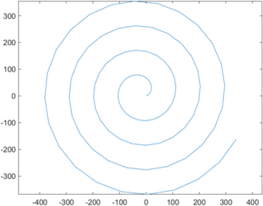
\includegraphics[width=.25\textwidth]{gfx/2021_02_turtle_examplespiral.png}
  }

    \item{\textbf{The House of Santa Claus:} The house of Santa Claus is a drawing game for children. The challenge is to draw a house in one line (without overlapping lines or lifting the pen). The resulting house looks like:

      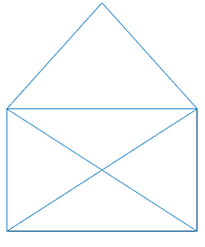
\includegraphics[width=.25\textwidth]{gfx/2021_02_turtle_houseofsanta.png}

      Implement a turtle proram (complete the given program) to draw such a house. Move the part drawing your turtle into a function called \code{house}.
      \begin{lstlisting}[language=matlab]

% call your own function house to draw a house
house()
plot(L(:,1), L(:,2))

function house()
% here put your turtle program calling move and turn
end
        
       \end{lstlisting}
      
    }
    \item{\textbf{Side-effect-Free House Function:}
      A common way of drawing the house starts in the bottom-left and ends in the bottom-right of the house. Now (allowing for lines on top of already existing lines), complete the function such that the turtle state is the same (same position, same direction) after running the function. Now, you can combine the \code{house} function with your alredy-programmed turtles.
      % squeeze in side-effect free and pure from functional programming
    }
    \item{\textbf{Function Parameters\up{*}:} Update your function to take a single parameter \code{size} that modulates the size of the house.
\begin{lstlisting}[language=matlab]
function house(size)
% here you can use size for computing the length of your move commands
end
\end{lstlisting}
    }

      \item{\textbf{Spirals of Houses\up+}. Use your side-effect-free function to draw spirals of houses. }

  \end{enumerate}

  \begin{solution}
    Under Construction
    \end{solution}

  
% TODO: let students implement two pen functions penup and pendown
  
\end{task}

%## Task 2.5: Turtle spirals (+)
%Draw a spiral of Santa Clauses houses.
%
%  
%
%
%
%  Read the blog given above. In this blog consisting of three articles, you are introduced to
%  functional programming using MATLAB anonymous functions.
%
%  \begin{itemize}
%  \item{Read about functional programmming, for example at \\
%    \url{https://en.wikipedia.org/wiki/Functional\_programming}}
%  \item{Inform yourself about anonymous functions and the varargin mechnaism for variable argument lists.}
%  \item{Recall the central idea of functional programming and think about its purpose, pros and cons.}
%  \item{Implement Euklids algorithm for the greatest common divisor. Therefore, complete the following
%    MATLAB file (Tip: The loop construct can easily be extended to a state holding a and b and the function
%    curly can be used to finally extract the second part of the state, which holds the result at the end
%    of the algorithm)
%%    \lstinputlisting{src/euklid/euklid_assignment.m}
%%    \url{https://github.com/mwernerds/big\_geospatial\_data\_lecture/blob/master/03\_matlab\_functional\_euklid/euklid\_assignment.m}
%
%  }
%  \end{itemize}
%  \begin{solution}
%    The following source code is an example of how to solve this problem:
%%    \lstinputlisting{src/euklid/euklid_solution.m}
%    An alternative solution uses the recur function and looks like
%    \begin{lstlisting}
%ggt = @(a,b) recur(...
%@(f,k,l) iif(l==0, k,...
%true, @() f(f,l, mod(k,l))), a,b);
%      \end{lstlisting}
%   \end{solution}
%\end{task}
%



\end{document}
